% this file is called up by the header file
% content in this file will be fed into the main document
% ----------------------- paths to graphics ------------------------
\graphicspath{{figures/}}

% ----------------------- contents start here ------------------------

                       
\chapter{Introduction}

Gaits are challenging and time-consuming to design manually.
To design effective gaits knowledge on expert level would be mandatory.
An alternative to solve this challenging task is to exploit machine learning techniques to evolve gaits on a robot.
In this case a genetic algorithm, which mimics natural selection in biological evolution, is well suited for selecting the best evolving gaits.
The goal is to learn a sequence of joint configurations on a robot's legs that lead to a preferably effective gait.
A genetic algorithm seems the logical choice for this complex task since it mimics the natural learning behavior.
A robot with legs learns to evolve gaits analog to animals.
In short, the idea is to evolve many generations of gaits in a simulation to get efficient forward-moving gaits on a quadrupedal robot, called ALLBOT (see figure \ref{fig:allbot}).

\begin{figure}[htb]
    \centering
    \begin{minipage}{.4\textwidth}
        \centering
        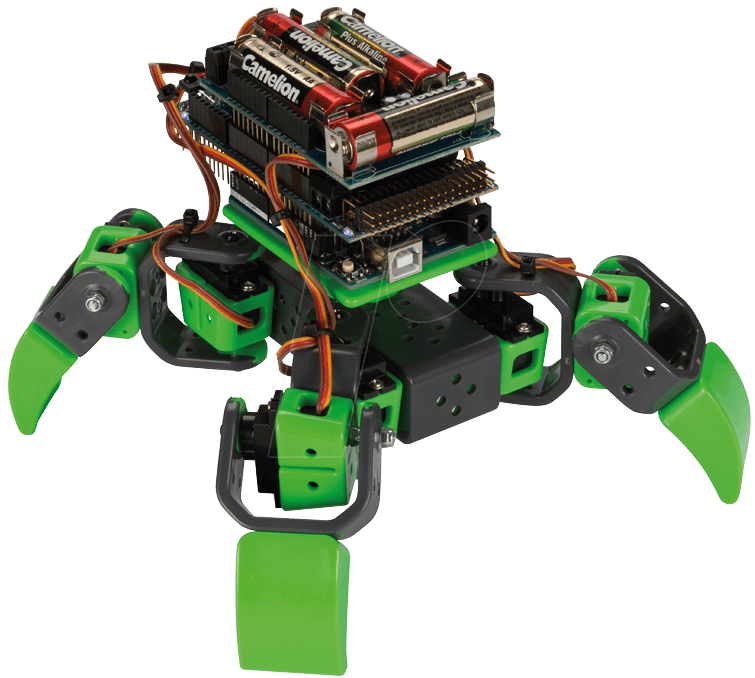
\includegraphics[width=\linewidth]{ALLBOT_4_LEG_01.png}
    \end{minipage}
    \hspace{.1\textwidth}
    \begin{minipage}{.4\textwidth}
        \centering
        %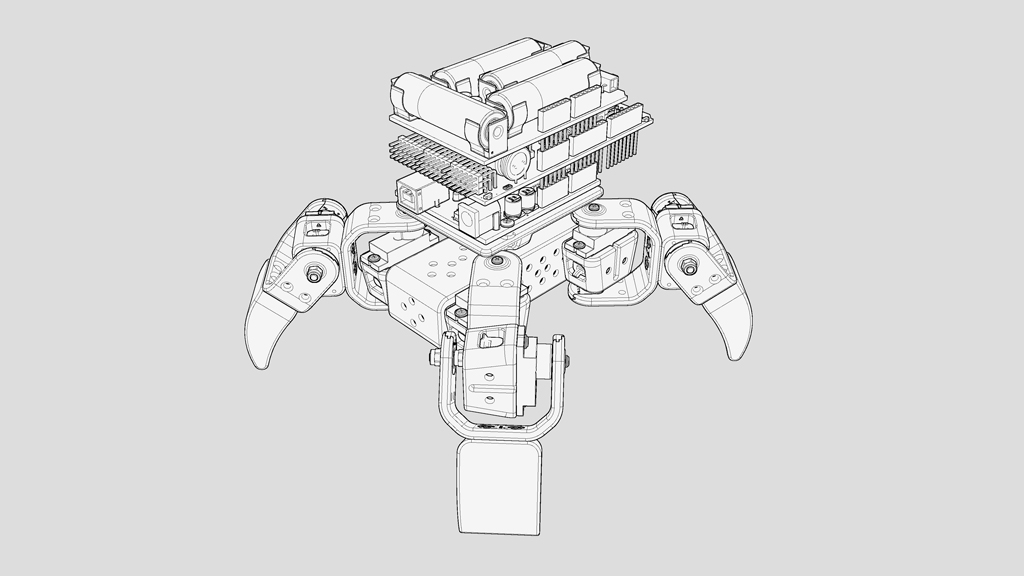
\includegraphics[width=\linewidth]{ALLBOT_isometric_2.jpg}
        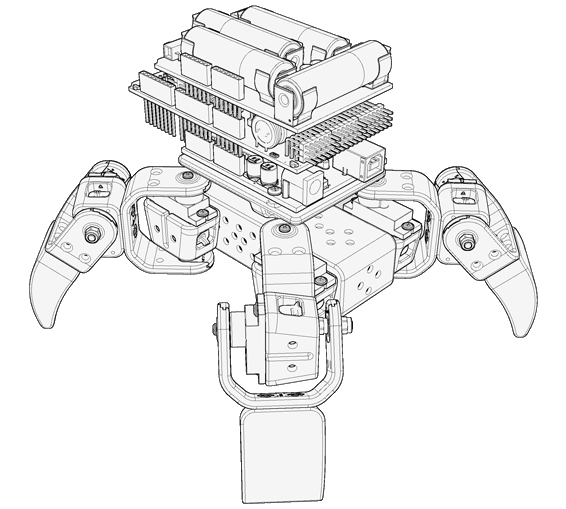
\includegraphics[width=\linewidth]{ALLBOT_isometric_2_bg_crop_flip.jpg}
    \end{minipage}
        \caption{ALLBOT robot (left) and an isometric representation (right).
                 Each leg has two servo actuated joints resulting in a total of eight degrees of freedom.
                 (sources: \url{https://cdn-reichelt.de/bilder/web/xxl_ws/C160/ALLBOT_4_LEG_01.png},
                 \url{http://www.allbot.eu/connect/manuals/})}
        \label{fig:allbot}
\end{figure}

This thesis is structured in the following manner:
First the ALLBOT robot is simulated with the robot simulation software Gazebo to avoid time-consuming training on the physical 
robot or suffering from mechanical failure during training. The simulation setup is described in chapter \ref{chap:simulation}.
Since the gaits are evolved with the deep learning genetic algorithm HyperNEAT, the theoretical background to HyperNEAT is summarized in chapter \ref{chap:hyperneat}.
The setup and parameters of the HyperNEAT algorithm as well as its implementation details are described in chapter \ref{chap:setup}.
Results are described in chapter \ref{chap:results} before conclusions are drawn in chapter \ref{chap:conclusion_outlook}.
